\documentclass[12pt, a4paper]{article}
\usepackage{caption}
\usepackage{subcaption,amsmath,siunitx}
\usepackage{natbib}
\usepackage{graphicx,mathtools}
\usepackage[english]{babel}
\usepackage[utf8]{inputenc}
\usepackage{fancyhdr}
\usepackage{amsmath}
\usepackage{mathtools}
\usepackage{tabto}
\usepackage{bm}
\usepackage{multirow}
\usepackage{float}
\usepackage{graphicx}
\usepackage{biblatex}
\addbibresource{ref.bib}
\graphicspath{{./images/}}
\newcommand*{\plogo}{\fbox{$\mathcal{PL}$}} % Generic dummy publisher logo
\usepackage[T1]{fontenc} % Output font encoding for international characters
\usepackage{stix} % Use the STIX fonts
\usepackage[font=small,labelfont=bf]{caption}
 
\begin{document}

\begin{titlepage} % Suppresses displaying the page number on the title page and the subsequent page counts as page 1
	
	\raggedleft % Right align the title page
	
	\rule{1pt}{\textheight} % Vertical line
	\hspace{0.05\textwidth} % Whitespace between the vertical line and title page text
	\parbox[b]{0.75\textwidth}{ % Paragraph box for holding the title page text, adjust the width to move the title page left or right on the page
		
		{\Huge\bfseries Eigenfaces vs. Fisherfaces:
        Recognition Using Class Specific Linear Projection}\\[2\baselineskip] % Title
		
		{\Large\textsc{Niraj Mahajan, Samarth Singh, Shaan Ul Haque}}\\[0.25\baselineskip]% Author name, lower case for consistent small caps
		
		{\large\textit{180050069, 180050090, 180070053}}\\[2\baselineskip] % Subtitle or further description
		
		{\Large\textsc{Course: CS663}}\\[0.5\baselineskip]
		
		{\Large\textsc{Instructors: Prof. Ajit Rajwade \& Prof. Suyash Awate}}
		\vspace{0.5\textheight} % Whitespace between the title block and the publisher
		
	}

\end{titlepage}
% \tableofcontents
\newpage

\textbf{Abstract -
In this implementation, we studied and implemented the Fischer Faces algorithm \cite{598228} which uses the technique of Linear Discriminant Analysis. We used several datasets and performed various face an feature recognition experiments to compare the performance of both these methods under varying image acquisition parameters like lighting, pose, expression.
}\\


\section{Introduction}
Algorithms such as eigen faces, correlation and linear subspaces take advantage of the fact that under admittedly idealized conditions,the variation within class lies in a linear subspace of the image space. Hence, the classes are convex and therefore linearly separable. One can perform dimensionality reduction using linear projection and still preserve linear separability. This is a strong argument in favor of using linear methods for dimensionality reduction in the face recognition problem, at least when one seeks insensitivity to lighting conditions.\\
Since the learning set is labeled, it makes sense to use this information to build a more
reliable method for reducing the dimensionality of the feature space. Here we argue that using class specific linear methods for dimensionality reduction and simple classifiers in
the reduced feature space, one gets better recognition rates than with either the Linear
Subspace method or the Eigenface method. Fisher's Linear Discriminant (FLD) is an
example of a \textit{class specific method}, in the sense that it tries to "shape" the scatter in order to make it more reliable for classification. This method selects transformation matrix in  in such a way that the ratio of the between-class scatter and the within-class scatter is maximized.\\
Let the between-class scatter matrix be defined as
\begin{equation*}
    S_{B} = \sum_{i=1}^{c} N_{i}(\boldsymbol{\mu} - \boldsymbol{\mu_{i}})(\boldsymbol{\mu} - \boldsymbol{\mu_{i}})^{T}
\end{equation*}
and the within-class scatter matrix be defined as 
\begin{equation*}
    S_{W} = \sum_{i=1}^{c}\sum_{x_k \epsilon X_i}^{}(\boldsymbol{x_k} - \boldsymbol{\mu_{i}})(\boldsymbol{x_k} - \boldsymbol{\mu_{i}})^{T}
\end{equation*}
where $\mu_i$ is the mean image of class $X_i$, and $N_i$ is the number of samples in class $X_i$. If $S_W$ is nonsingular, the optimal projection $W_{opt}$ is chosen as the matrix with orthonormal columns which maximizes the ratio of the determinant of the between-class scatter matrix of the projected samples to the determinant of the within-class scatter matrix of the
projected samples, i.e.
\begin{flalign*}
    W_{opt} &= \underset{W}{\operatorname{argmax}}  \frac{|W^TS_BW|}{|W^TS_WW|}\\
    &= [\boldsymbol{w_1} \boldsymbol{w_2} \ ...\  \boldsymbol{w_m}]
\end{flalign*}
where \{$w_i$ | i = 1, 2, . . .m\} is the set of generalized eigenvectors of $S_B$ and $S_W$ corresponding to the m largest generalized eigenvalues \{$\lambda_i$ | i = 1, 2, ... m\}, i.e.
\begin{flalign*}
    S_B\boldsymbol{w_i} = \lambda_i S_w\boldsymbol{w_i}
\end{flalign*}
To illustrate the advantage of Fischer Faces, we have provided with a figure taken from the paper.
\begin{figure}[htb]
    \centering
    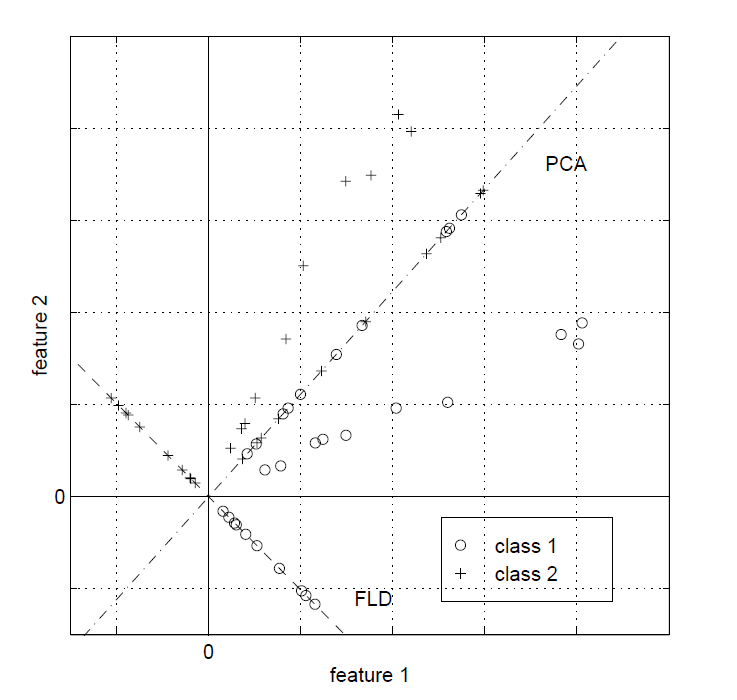
\includegraphics[width = 0.6\linewidth]{Screenshot (290).png}
    \caption{A comparison of principal component analysis (PCA) and Fisher's linear discriminant (FLD) for a two class problem where data for each class lies near a linear subspace.}
\end{figure}

In the face recognition problem one is confronted with the difficulty that the within class
scatter matrix $S_W \ \epsilon \ R^{n\times n}$ is always singular. This stems from the fact that the rank of $S_W$ is at most N-c, and in general, the number of images in the learning set N is much smaller than the number of pixels in each image n. This means that it is possible to choose the matrix W such that the within-class scatter of the projected samples can be made exactly zero.\\
In order to overcome the complication of a singular $S_W$, we propose an alternative
to the criterion. This method, which we call Fisherfaces, avoids this problem by
projecting the image set to a lower dimensional space so that the resulting within-class
scatter matrix $S_W$ is nonsingular. This is achieved by using PCA to reduce the dimension
of the feature space to N-c and then, applying the standard FLD reduce the dimension to c-1. More formally, $W_{opt}$ is given by:
\begin{flalign*}
    W_{opt}^T = W_{fld}^TW_{pca}^T
\end{flalign*}
where
\begin{flalign*}
    W_{pca} &= \underset{W}{\operatorname{argmax}}  |W^TS_TW|\\
    W_{fld} &= \underset{W}{\operatorname{argmax}} \frac{|W^TW_{pca}^TS_BW_{pca}W|}{|W^TW_{pca^T}S_WW_{pca}W|}
\end{flalign*}
here, $S_T$ is the Scatter Matrix given by:
\begin{flalign*}
    S_T = \sum_{k=1}^{N} (\boldsymbol{x_k} - \boldsymbol{\mu})(\boldsymbol{x_k} - \boldsymbol{\mu})^{T}
\end{flalign*}
Note that the optimization for $W_{pca}$ is performed over $n\times(N-c)$ matrices with orthonormal columns, while the optimization for $W_{fld}$ is performed over $(N-c)\times m$ matrices with orthonormal columns. In computing $W_{pca}$ we have thrown away only the smallest c principal components.
\section{Analysis of Experimental Results}
In this section we performed face recognition and glasses recognition experiments on the CMU Face dataset\cite{cmu}, Yale dataset A, and Yale dataset B\cite{yaleB}. We performed a random 40-60 split for testing-training datasets and performed face recognition on all three datasets. We also performed a glasses recognition experiment on the YaleB dataset using the "leaving one out" algorithm\cite{nla.cat-vn430142}.
\subsection{Face Recognition}
\begin{table}[H]
    \centering
    \begin{tabular}{ |p{4.1cm}|p{2.5cm}|p{2.5cm}|p{2.5cm}|  }
 \hline
\multirow{2}{0.1cm}{Method} & \multicolumn{3}{c|}{Error Rate (in \%)} \\
 \cline{2-4}
   &   CMU Face & YaleA & YaleB \\
 \hline
 Eigen Faces & 0.91 & 16.67 & 45.85 \\
 \hline
 Eigen Faces \newline (w/o top 3 eigvectors) & 1.82 & 13.33 & 20.24 \\
 \hline
 Fischer Faces & 38.64 & 1.67 & 5.87 \\
 \hline
\end{tabular}
    \caption{Error Rates of Face Recognition}
    \label{tab:face_recog}
\end{table}

\subsubsection{Yale A Face Database}
The yale A dataset contains 165 grayscale images in GIF format of 15 individuals.There are 11 images per subject, one per different facial expression or configuration: center-light, w/glasses, happy, left-light, w/no glasses, normal, right-light, sad, sleepy, surprised, and wink.
We applied the fischer-face algorithm, reducing the dimensionality to 15 and the eigen-face algorithm, reducing the dimensionality to 30. \\ Since this dataset has some images with varying illumination, it is obvious that the fischer-face algorithm will outperform the eigen-face algorithm (table \ref{tab:face_recog}). Note that the error for the eigen-face algorithm is much higher when we do not remove the top 3 eigenvectors. This is because the face images follow a lambertian model and lighting variation can be represented in a rank 3 space. (the variation in the images due to lighting changes is much higher compared to pose and expression changes.)

\subsubsection{Yale B Face Database}
The Yale Face Database B contains 2415 images of 38 human subjects under varying 64 illumination conditions. 
We applied the fischer-face algorithm, reducing the dimensionality to 38 (number of classes) and the eigen-face algorithm, reducing the dimensionality to 50. \\ Since this dataset has images with just varying illuminations, the fischer-face algorithm will again outperform the eigen-face algorithm (table \ref{tab:face_recog}). Again, the error for the eigen-face algorithm is much higher when we do not remove the top 3 eigenvectors.

\subsubsection{CMU Face Database}
The CMU database consists of 20 classes each class containing 32, 128*120 .pgm format, pictures of a person in different orientation (i.e. left faced, right faced, straight and up), different expressions (i.e. angry, happy, neutral and sad) and with/without glasses. Pictures were not cropped and conatined a lot of background in them. \\
We divided the dataset into 70-30 ratio by randomly selecting 70\% of each class for training and 30\% for testing.  We applied the fischer face (reducing the dimensionality to 19) and eigen face (reducing the dimensionality to 19) algorithm to this CMU Face dataset.
Eigen Faces was far better than Fischer Faces (table \ref{tab:face_recog}). This unexpected result was due to two reasons:
\begin{itemize}
    \item Change in Face Alignment - Changing Face Alignment breaks the assumption of high linear separability. Since Linear Discriminant Analysis ignores highly changing features of a face, changing alignment induces excessive variation in face leading the algorithm to neglect whole face. Thus, we see a lot of error in face recognition when Fischer faces method is used.
    \item Non-cropped Images - Even when only frontal images are used results for Eigen Faces are better than Fischer Faces because Fischer Face neglects features of an image which vary a lot(such as eyes, mouth, face alignment, etc) and gives a lot of weightage to background due to its non variability and thus losing important information regarding the face. 
\end{itemize}
\subsection{Glasses Recognition}
\begin{table}[H]
    \centering
    \begin{tabular}{ |p{4.1cm}|p{6.5cm}|  }
 \hline
 Method & Error Rate (in \%) for YaleA  \\
 \hline
 Eigen Faces & 40.00 \\
 \hline
 Eigen Faces \newline (w/o top 3 eigvectors) & 53.33 \\
 \hline
 Fischer Faces & 33.33 \\
 \hline
\end{tabular}
    \caption{Error Rates of Glasses Recognition}
    \label{tab:glasses_recog}
\end{table}
In this section we perform glasses recognition on the Yale A dataset. \\
The yale A dataset contains images of 15 individuals, each with and without glasses. Hence we can use these 30 images to train and test a fischerfaces algorithm on this data and compare the results with the eigenfaces algorithm \\

We applied the fischer-face algorithm, reducing the dimensionality to 1 and the eigen-face algorithm, reducing the dimensionality to 10. \\ 
Our task involves a binary classification over multiple people. Hence the fischerface algorithm is bound to outperform the eigenface algorithm (table \ref{tab:glasses_recog}), since the eigenface algorithm will give a high variance for different people. Since this dataset has no illumination or pose variation, removing the top3 eigenvectors will lead to loss of vital data, and this too will decrease the accuracy. Also, we notice that compared to the error rate in face recognition, the error rate for glasses recognition using the fischer method is high. This is because our dataset is really small (just 30 images). But still, the relative magnitudes of the accuracy are as per our expectation and have been explained.
\newpage
\section{Conclusion}
We thus conclude that the Fisherface method appears to be the best at extrapolating and interpolating over variation in lighting. \\ Removing the largest three principal components does improve the performance of the Eigenface method in the presence of lighting variation, but harms the accuracy if lighting variations are not present. The Fisherface method appears to be the best at simultaneously handling variation in lighting and expression. Also, the fischerface method tries to ignore the features within the same class that have high variances.
\section{Usage of Code}
\begin{itemize}
    \item Run the files \textbf{yaleA\_tester.py}, \textbf{yaleB\_tester.py}, \textbf{cmu\_tester.py} (in cmu\_codes directory)
    \item Download the data and place it in the datasets folder. Refer https://www.cse.iitb.ac.in/~nirajm/shared/663datalinks.txt for more details
\end{itemize}
\newpage
\printbibliography


\end{document}
